\chapter{Name Resolution}
\label{ch:name_resolution}

\section{Overview}
\label{sec:resolution_overview}

The name resolution phase transforms the symbolic type references
($\tau = \texttt{Unresolved}$) produced by the extraction phase into
semantically resolved pointers. Formally:
$$\rho : \mathcal{D} \to \mathcal{D}_{\text{res}}$$
where $\mathcal{D}$ is the domain of extracted module hierarchies
$\vec{\mathcal{M}}$,
and $\mathcal{D}_{\text{res}}$ represents the domain of semantically
resolved module
trees. The transformation preserves the isomorphic structural
topology of the codebase,
while type references undergo a state transition: every
\texttt{TypeRef::Unresolved} is
lowered through the Query Algebra ($\mathcal{Q}$) and evaluated into
one of the six
terminal or compound post-resolution states (as formalized in Chapter
  \ref{ch:ir_formalization}
and Chapter \ref{ch:analysis_process}): \texttt{Resolved}, \texttt{External},
\texttt{Primitive}, \texttt{Union}, \texttt{EvaluatedAccess}, or
\texttt{Failed}.
This phase operates entirely on the IR domain and is independent of
the source language.

The resolution operator is decomposed into two algebraic sub-phases:
$$\rho = \rho_{\text{exec}} \circ \rho_{\text{build}}$$
\begin{enumerate}
  \item \textbf{Query Building} ($\rho_{\text{build}}$): Traverses the module
    hierarchy with a local \textit{Symbol Stack} ($\Delta$), replacing
    raw \texttt{Unresolved} paths with algebraic
    \texttt{ResolutionQuery} expressions ($q \in \mathcal{Q}$).
  \item \textbf{Query Execution} ($\rho_{\text{exec}}$): Builds a global
    \textit{Scope Tree} ($\mathcal{E}$) from the entire workspace and
    evaluates all query expressions against the immutable Execution Context
    $\Gamma = \langle \mathcal{E}, \mathcal{P}, \mathcal{K} \rangle$.
\end{enumerate}

In classical compiler construction and program analysis, resolving
symbolic names across
heterogeneous source files presents substantial theoretical and
practical hurdles due to forward
references, cyclic module imports, and diverse lexical scoping
conventions. In recent formal
language engineering, language-independent name binding has been
grounded in the theory of
\textit{Scope Graphs} \cite{zwaan_scope_2023} and industrially scaled
in GitHub's \textit{Stack Graphs}
\cite{creager_stack_2023}, both of which abstract name resolution as
generalized path-finding
over graph-structured lexical scopes.

OmniDeps adopts a pragmatic, two-phase algebraic formulation
specifically optimized for
static architectural dependency analysis. Rather than resolving raw
strings eagerly during
file parsing or constructing monolithic global constraint systems:
\begin{itemize}
  \item \textbf{Decoupling Intra-procedural State
    ($\rho_{\text{build}}$)}: During syntactic
    extraction (Phase 1), analysis is strictly isolated file-by-file
    without visibility into
    external units. The query building phase resolves local concerns
    (formal parameter types,
    local variables, and block-level lexical shadowing). By rewriting
    syntactic references into
    self-contained algebraic formulas $q \in \mathcal{Q}$,
    $\rho_{\text{build}}$ eliminates all
    transient intra-procedural state. Once this phase completes, the
    Symbol Stack is safely
    deallocated, and all method bodies are represented uniformly by
    closed algebraic expressions.
  \item \textbf{Global Topological Resolution
    ($\rho_{\text{exec}}$)}: Because intra-procedural
    substitutions have already taken place, the execution engine
    receives pure navigation formulas.
    Operating on the unified workspace Scope Tree $\mathcal{E}$,
    $\rho_{\text{exec}}$ handles
    inter-procedural references, cross-module imports, and class
    inheritance hierarchies in a single,
    well-defined topological traversal, completely unencumbered by
    source file ordering or local
    lexical complexities.
\end{itemize}

Figure \ref{fig:two_phase_resolution} summarizes the operational flow between these two phases.

\begin{figure}[htpb]
  \centering
  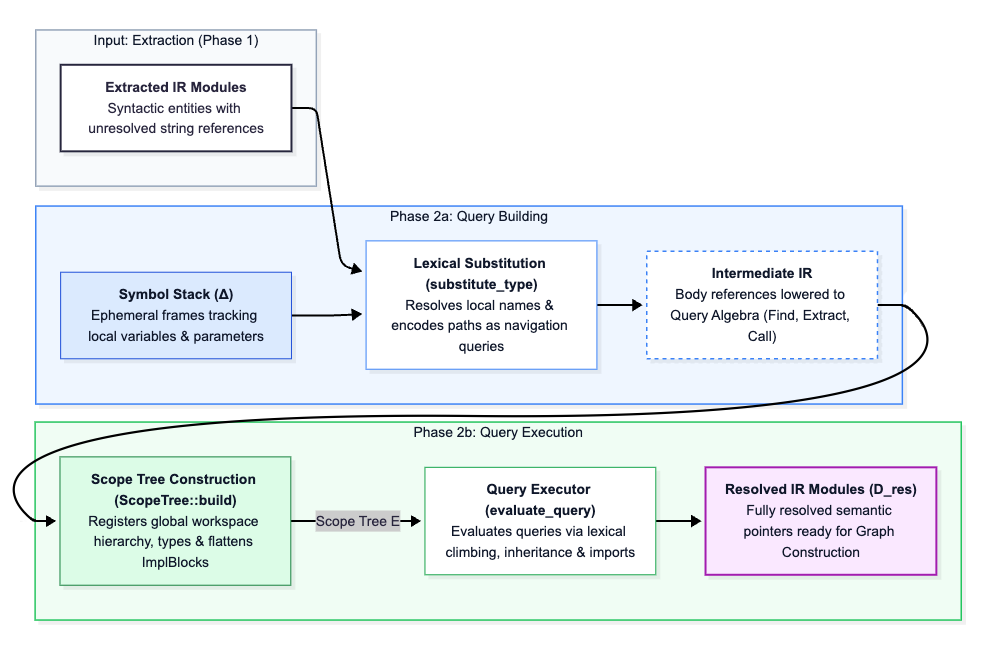
\includegraphics[width=\textwidth]{images/name_resolution/two_phase_resolution.png}
  \caption{Two-phase resolution architecture: query building ($\rho_{\text{build}}$) transforms AST paths into algebraic queries using the local Symbol Stack ($\Delta$), while query execution ($\rho_{\text{exec}}$) evaluates queries across the global Scope Tree ($\mathcal{E}$).}
  \label{fig:two_phase_resolution}
\end{figure}

\section{The Query Algebra ($\mathcal{Q}$)}
\label{sec:query_algebra}

Rather than resolving raw strings eagerly, the system encodes
resolution intent as an algebraic formula $\mathcal{Q}$ composed of
three navigation primitives:

\begin{itemize}
  \item $\texttt{Find}(\iota)$: \textbf{Ascending search}. Starting from
    the current lexical scope, climb up the scope tree until a symbol
    named $\iota \in \mathcal{I}$ is found. This models lexical scope
    resolution, where a
    name is first searched locally, then in enclosing scopes, then globally.
  \item $\texttt{Extract}(q, \iota)$: \textbf{Structural member descent}.
    Evaluate sub-query $q$ to obtain a scope (a module or a type),
    then search for member $\iota \in \mathcal{I}$ within that scope,
    including inherited
    members from super-types. This models qualified access paths such
    as \texttt{obj.field}, \texttt{Module::Type}, or \texttt{package.Class}.
  \item $\texttt{Call}(q)$: \textbf{Transitive invocation / Return
    type evaluation}.
    Evaluate sub-query $q$ to obtain a callable symbol (function,
    method, or constructor),
    then resolve to its declared or inferred return type. This models
    return type propagation
    during local variable type inference (e.g., \texttt{let x = f()})
    as well as fluent
    method chaining patterns where the returned instance serves as
    the receiver of a subsequent member access.
\end{itemize}

These three primitives are sufficient to encode the resolution intent
of any type reference that appears in practice. Table
\ref{tab:query_examples} illustrates several representative encodings.

\begin{table}[htpb]
  \centering
  \small
  \begin{tabular}{|l|l|}
    \hline
    \textbf{Source Expression} & \textbf{Type-Level Query Encoding} \\ \hline
    \texttt{Foo} & $\texttt{Find}(\texttt{Foo})$ \\ \hline
    \texttt{a.b.T} &
    $\texttt{Extract}(\texttt{Extract}(\texttt{Find}(\texttt{a}),
    \texttt{b}), \texttt{T})$ \\ \hline
    \texttt{foo()} (return type) &
    $\texttt{Call}(\texttt{Find}(\texttt{foo}))$ \\ \hline
    \texttt{obj.method()} (return type) &
    $\texttt{Call}(\texttt{Extract}(\texttt{Find}(\texttt{obj}),
    \texttt{method}))$ \\ \hline
    \texttt{a.f().g()} &
    $\texttt{Call}(\texttt{Extract}(\texttt{Call}(\texttt{Extract}(\texttt{Find}(\texttt{a}),
    \texttt{f})), \texttt{g}))$ \\ \hline
  \end{tabular}
  \caption{Examples of source expressions and their corresponding
  query algebra encodings for type inference and member chaining.}
  \label{tab:query_examples}
\end{table}

A crucial architectural distinction must be emphasized between
\textit{behavioral invocation dependencies}
and \textit{type-level invocation queries}:
\begin{itemize}
  \item In call graph construction (Phase 3), a function call
    statement in a block body
    (e.g., \texttt{validate()}) constitutes a control-flow coupling.
    Here, the target of the call
    must resolve to the \textbf{callable entity itself}
    ($\texttt{Find}(\texttt{validate})$),
    allowing OmniDeps to emit a direct $\texttt{Calls}$ edge between
    the caller and the callee.
    Wrapping such statements in $\texttt{Call}(\cdot)$ would evaluate
    their return type (yielding
    e.g. \texttt{void} or \texttt{bool}), which would erroneously
    redirect call edges to return types.
  \item In contrast, the algebraic constructor $\texttt{Call}(q)$ is
    utilized strictly in
    \textbf{type inference contexts}: when an untyped local variable
    is initialized with a function call
    (\texttt{let x = build()}) or when chaining member accesses
    across invocations (\texttt{conn.get().open()}).
\end{itemize}

\section{Phase 2a: Query Building ($\rho_{\text{build}}$)}
\label{sec:query_building}

The first sub-phase traverses the extracted module hierarchy and
transforms every \texttt{TypeRef::Unresolved} into a
\texttt{TypeRef::ResolutionQuery}. The transformation is performed by
the function \texttt{substitute\_type}, which applies the
\textit{Symbol Stack} ($\Delta$) to resolve local variable references
and encode the remaining path segments as \texttt{Extract} and
\texttt{Call} queries.

\subsection{The Symbol Stack ($\Delta$)}

The Symbol Stack is an ephemeral lexical environment that tracks
local variable and parameter bindings within function scopes, adhering to
the classical compiler formulation of block-structured lexical environments
with scoped symbol tables \cite{aho_compilers_2007}. It is structured as a
stack of frames:
$$\Delta = [\delta_1, \delta_2, \ldots, \delta_n] \quad \text{where}
\quad \delta_i : \mathcal{I} \to \mathcal{Q}$$

Each frame $\delta_i$ maps identifier names $\iota \in \mathcal{I}$
to their corresponding
query expressions. Frames are pushed when entering a function or
block scope, and popped when exiting. Lookup proceeds from the top of
the stack downward (most-recently-pushed frame $\delta_n$ first),
naturally modeling
lexical shadowing.

\subsection{The Substitution Algorithm}

The lexical substitution procedure transforms unresolved syntactic
references into
algebraic queries via the function \texttt{substitute\_type(ctx, tr,
is\_call)}. When encountering
a \texttt{TypeRef::Unresolved} consisting of a qualified path $\pi =
\langle \iota_1, \iota_2, \ldots, \iota_k \rangle$,
the builder proceeds as follows:
\begin{enumerate}
  \item \textbf{Base Identifier Resolution}: Look up the leading
    segment $\iota_1$ in the Symbol Stack $\Delta$
    (iterating through frames from $\delta_n$ down to $\delta_1$).
    If a local binding exists ($\iota_1 \mapsto q_{\text{local}}$),
    adopt $q_{\text{local}}$ as the base query;
    otherwise, emit an ascending lexical search $\texttt{Find}(\iota_1)$.
  \item \textbf{Structural Member Chaining}: For each subsequent
    segment $\iota_j$ ($j > 1$), wrap the
    accumulated query into a member extraction:
    $$q \leftarrow \texttt{Extract}(q, \iota_j)$$
  \item \textbf{Contextual Invocation Wrapping}: The Boolean flag
    \texttt{is\_call} specifies whether the
    reference is evaluated as a return-type query:
    \begin{itemize}
      \item For references representing \textit{behavioral invocation
        targets} ($c \in b.\text{calls}$),
        \textit{instantiations} ($i \in b.\text{instantiates}$), and
        \textit{direct accesses}
        ($a \in b.\text{accesses}$), the builder invokes
        \texttt{substitute\_type} with $\texttt{is\_call} = \text{false}$.
        The query directly targets the callee symbol or accessed
        member, preserving the target's identity
        for call graph edge creation.
      \item When a call expression serves as a value provider in
        variable type inference
        (e.g., extracting the inferred type of an untyped local
          declaration $x = f()$ in
        Section \ref{sec:heuristics}), the resulting query is wrapped
        in $\texttt{Call}(\cdot)$
        (i.e., $q \leftarrow \texttt{Call}(q)$), signaling the
        executor to unpack the callee's return type.
    \end{itemize}
\end{enumerate}

For \texttt{TypeRef::Union} variants, the substitution is applied
recursively to each member of the union.

\subsection{Variable and Parameter Binding}

As the builder traverses function bodies, it pushes bindings onto the
Symbol Stack:

\begin{itemize}
  \item \textbf{Parameters}: For each parameter with identifier
    $\iota_{\text{param}}$ and declared type $\tau$,
    the type is transformed via $\rho_{\text{build}}$:
    $$q_\tau = \text{substitute\_type}(\text{ctx}, \tau, \text{false})$$
    If $q_\tau$ evaluates to a \texttt{ResolutionQuery}, the binding
    $\iota_{\text{param}} \mapsto q_\tau$
    is registered in the current frame $\delta_n$. For variadic
    parameters and parameters with failed type extraction,
    no binding is pushed.
  \item \textbf{Local Variables}: For each local variable declaration
    $\iota_{\text{var}}$
    in a block with declared or inferred type $\tau$, the type is
    similarly substituted into $q_\tau$.
    If $q_\tau \in \mathcal{Q}$, the binding $\iota_{\text{var}}
    \mapsto q_\tau$ is pushed into the top frame $\delta_n$.
  \item \textbf{Block Scoping}: When entering a sub-block (an
    \texttt{if}, \texttt{while}, or anonymous scope), a fresh frame
    $\delta_{n+1}$ is
    pushed onto $\Delta$. When exiting, the frame is popped. This
    correctly models
    lexical scoping, where a variable declared in an inner block
    shadows one in an outer block but does not outlive it.
\end{itemize}

\subsubsection{Implicit Self/This Injection}

For languages with an implicit receiver parameter, the builder
injects special bindings based on the language configuration:
\begin{itemize}
  \item If \texttt{self\_keyword} is set (e.g., \texttt{"self"} for
    Rust, \texttt{"this"} for Java/C++), a binding $kw \mapsto q_{\text{self}}$
    is pushed when entering a method scope, where $q_{\text{self}}$
    is the query targeting
    the enclosing structured type.
  \item If \texttt{implicit\_first\_param\_as\_self} is true
    (Python), the first parameter of each method (typically named
    \texttt{self}) is automatically bound to the enclosing class,
    regardless of its declared type.
\end{itemize}

This mechanism is what allows references like \texttt{self.field} or
\texttt{this.method()} to be correctly resolved to members of the
enclosing type.

\subsection{Output of Phase 2a}

At the end of the query building phase, the Symbol Stack is
destroyed. Intra-procedural type references in the IR are now:
\begin{itemize}
  \item \texttt{TypeRef::ResolutionQuery($q$)}: An algebraic
    expression ready for global evaluation against the Scope Tree.
  \item Composite type structures (\texttt{Generic}, \texttt{TypeVar},
    \texttt{Union}, and \texttt{EvaluatedAccess}) whose constituent
    references contain substituted queries.
\end{itemize}

No raw local identifiers remain in executable blocks.
The classification of built-in primitive types and the identification of
unresolvable symbols are deliberately deferred to Phase 2b, where they are
evaluated globally against the Primitive Registry ($\mathcal{P}$) and the
Scope Tree ($\mathcal{E}$).

\section{Phase 2b: Query Execution ($\rho_{\text{exec}}$)}
\label{sec:query_execution}

The second sub-phase builds a global Scope Tree from the entire
workspace and evaluates all \texttt{ResolutionQuery} expressions. The
key property of this phase is that it runs \textbf{after} the entire
workspace has been parsed into memory, making source file order and
forward references irrelevant.

\subsection{The Scope Tree ($\mathcal{E}$)}
\label{sec:scope_tree}

The Scope Tree is a hierarchical data structure that mirrors the
lexical scoping rules of the source code. Each scope represents a
named lexical environment (a module, a class, a function, or a block)
and contains a symbol table mapping identifiers to their semantic roles.

Unlike the generalized, unguided graph traversal algorithms employed by
Stack Graphs \cite{creager_stack_2023}, which can experience severe
combinatorial path-explosion during whole-program dependency extraction
(as discussed in Chapter \ref{ch:related_work}), the Scope Tree $\mathcal{E}$
models the workspace as a deterministic, single-parent lexical hierarchy.
Lexical climbing for $\texttt{Find}$ ascends deterministically toward the root,
while member descent for $\texttt{Extract}$ follows unambiguous nominal
containment. By restricting name navigation to this deterministic tree
topology, OmniDeps completely avoids non-deterministic path exploration.

\subsubsection{Arena Allocator Implementation}

The Scope Tree is implemented using an \textbf{Arena Allocator}
pattern: all scopes reside in a contiguous flat vector
(\texttt{Vec<Scope>}), indexed by integer \texttt{ScopeId} values
(\texttt{type ScopeId = usize}). Each \texttt{Scope} structure contains:

\begin{itemize}
  \item \texttt{id: ScopeId}: The scope's index in the arena.
  \item \texttt{parent: Option<ScopeId>}: A pointer to the enclosing scope.
  \item \texttt{name: String}: The scope's identifier (e.g., the
    module name, the class name).
  \item \texttt{symbols: HashMap<String, Symbol>}: The symbol table.
  \item \texttt{imports: Vec<Import>}: The import declarations
    visible in this scope.
  \item \texttt{super\_types: Vec<TypeRef>}: The inheritance or trait
    implementation references (for type scopes).
  \item \texttt{is\_module: bool}: Whether this scope represents a
    module (affects import resolution behavior).
  \item \texttt{language: Option<String>}: The language of the module
    (for configuration lookup).
  \item \texttt{type\_parameters: Vec<String>}: The formal generic type parameter
    names declared by the scope (used for type substitution).
  \item \texttt{is\_phantom: bool}: Indicates whether this scope is a synthetic
    phantom scope introduced for a generic type parameter.
\end{itemize}

The \texttt{Symbol} enum distinguishes four kinds of entries:
\begin{itemize}
  \item \texttt{Module(ScopeId)}: A sub-module, pointing to its scope.
  \item \texttt{Type(ScopeId)}: A structured type (class, struct,
    interface, trait), pointing to its scope.
  \item \texttt{TypeAlias(TypeRef)}: A type alias, storing its target reference.
  \item \texttt{Value(TypeRef)}: A concrete value (field, function,
    parameter, local variable), storing its type reference.
\end{itemize}

The Arena Allocator pattern represents a fundamental systems-level
architectural choice
in OmniDeps. In garbage-collected languages, hierarchical scope
structures are typically modeled
using bidirectional object references between parent and child
scopes. In Rust, replicating
such pointer graphs naively would necessitate shared mutable pointer
cycles, such as
\texttt{Rc<RefCell<Scope>>}. This introduces several critical limitations:
\begin{enumerate}
  \item \textbf{Memory Leaks via Reference Cycles}: Bidirectional
    links between parent scopes
    and child scopes naturally create strong reference cycles that
    prevent automated deallocation,
    requiring fragile manual cleanup routines or complex weak pointer
    schemes (\texttt{Weak<RefCell<Scope>>}).
  \item \textbf{Borrow Checker Violations and Runtime Overhead}:
    Climbing parent scopes
    or inspecting enclosing lexical frames during recursive
    traversals would trigger dynamic borrow
    checking (\texttt{RefCell::borrow\_mut}), introducing runtime
    performance penalties and the
    constant hazard of runtime panics due to conflicting concurrent borrows.
  \item \textbf{Cache Locality}: Heap-allocated node graphs scatter
    individual scope structures across
    disjoint memory regions, degrading CPU cache line utilization
    during intensive symbol lookup phases.
\end{enumerate}

By storing all scopes in a flat, contiguous vector
(\texttt{Vec<Scope>}) and modeling pointers
as plain scalar indices (\texttt{type ScopeId = usize}), the Arena
Allocator completely decouples
lexical graph topology from Rust's memory ownership model:
\begin{itemize}
  \item The entire Scope Tree $\mathcal{E}$ is owned by a single
    contiguous memory container
    with $O(1)$ amortized allocation and deterministic deallocation,
    completely eliminating reference counting overhead;
  \item The parent relation \texttt{parent: Option<ScopeId>} is a
    primitive 64-bit integer,
    inherently immune to circular reference memory leaks;
  \item Traversal algorithms can simultaneously borrow the arena
    immutably while traversing parent
    and child indices freely, ensuring absolute compile-time memory
    safety without locks or runtime checks;
  \item Canonical path reconstruction (computing the fully qualified
    path $\pi$ of any entity)
    is achieved by climbing ancestor \texttt{ScopeId} integers with
    zero pointer chasing overhead.
\end{itemize}

Figure \ref{fig:scope_tree_arena} illustrates this arena-allocated topology.

\begin{figure}[htpb]
  \centering
  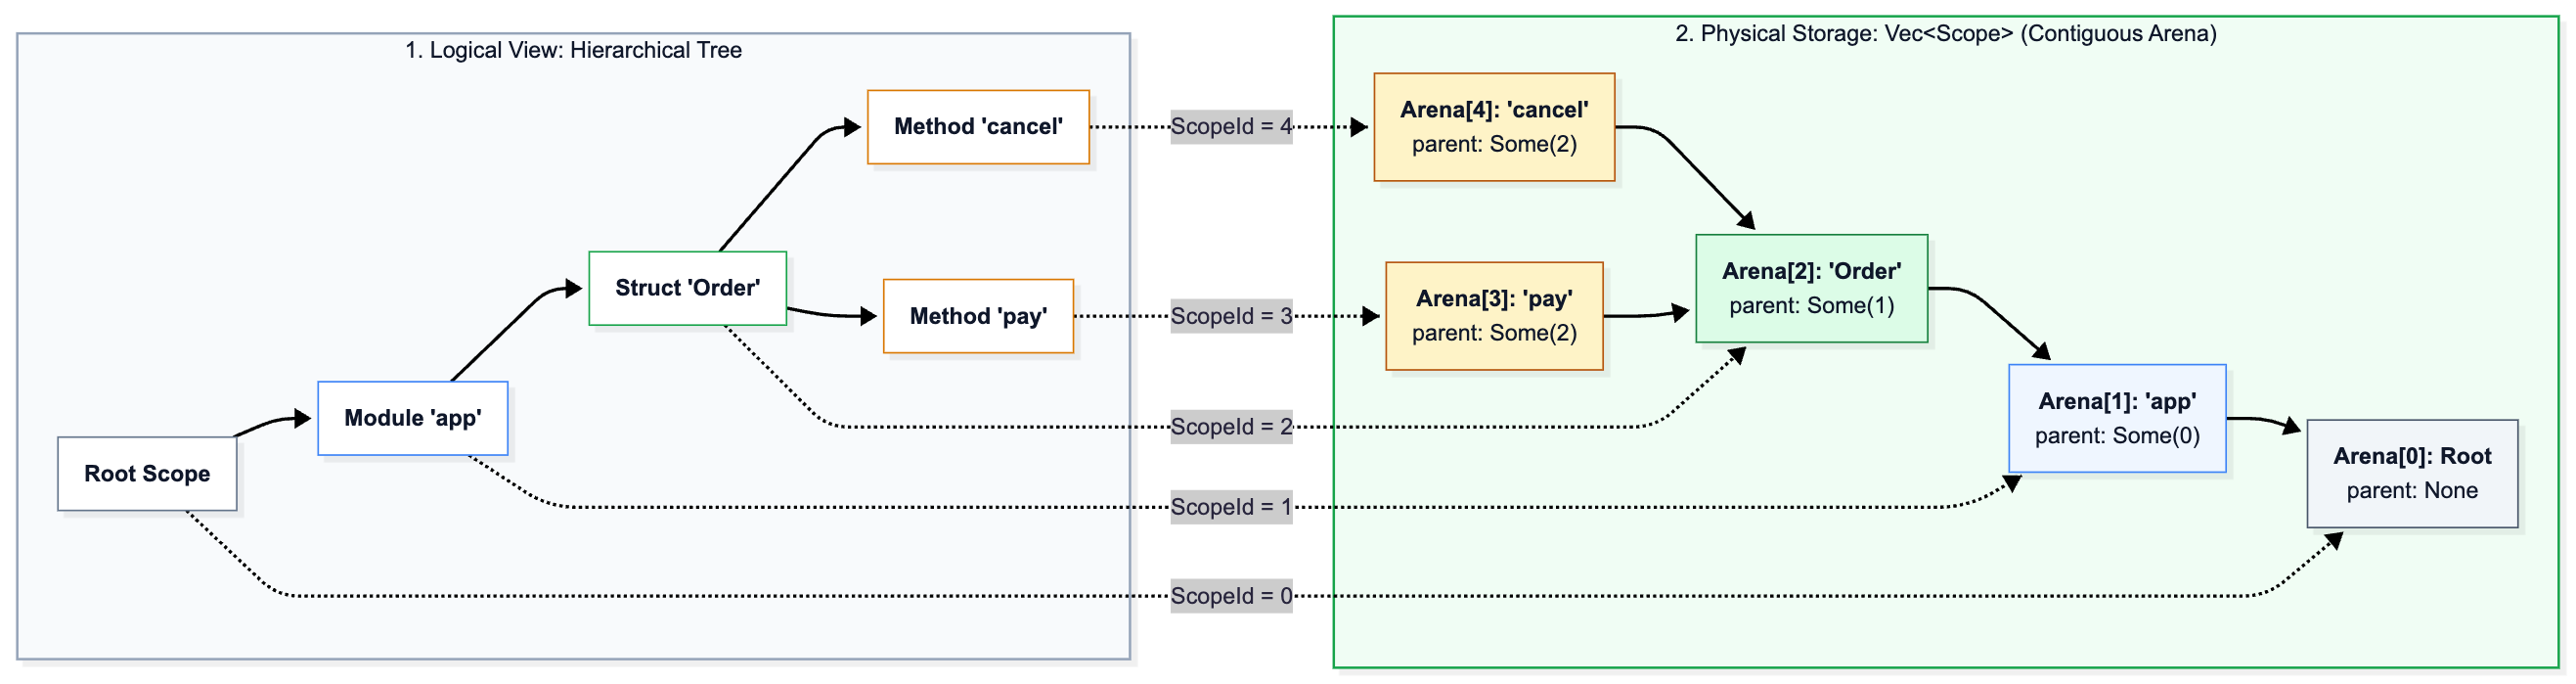
\includegraphics[width=\textwidth]{images/name_resolution/scope_tree_arena.png}
  \caption{Contiguous arena layout of the Scope Tree: scopes reside linearly in \texttt{Vec<Scope>} indexed by integer \texttt{ScopeId}, with parent relations modeled as scalar integers to eliminate pointer cycles.}
  \label{fig:scope_tree_arena}
\end{figure}

\subsubsection{Scope Tree Construction}

The Scope Tree is constructed by the function
\texttt{ScopeTree::build}, which recursively registers all components
from the workspace modules:

\begin{enumerate}
  \item \textbf{Root}: A root scope (id: 0, name: \texttt{"root"}) is created.
  \item \textbf{Modules}: \texttt{register\_module} walks module
    paths, creating intermediate module scopes or merging with
    existing ones (if the same module path was contributed by
    multiple files). Imports, type aliases, structured types, free
    functions, free variables, and sub-modules are registered within
    the module scope.
  \item \textbf{Structured Types}:
    \texttt{register\_structured\_type} creates a type scope,
    registers fields as \texttt{Symbol::Value}, records super-types, and
    recursively handles nested types. Methods are registered as callable
    symbols in the class scope. Constructors and destructors
    are excluded from the class's dynamic symbol lookup table to prevent
    shadowing the nominal type of the class during base-class climbing
    in object-oriented languages (such as C++). Instead, constructors
    and destructors are registered as independent sub-scopes and linked
    via structural \texttt{NestedIn} relationships, ensuring that their
    parameters, bodies, and calls are fully analyzed without contaminating
    type queries.
  \item \textbf{Type Parameters and Phantom Scopes}:
    When registering a generic structured type or function,
    \texttt{register\_structured\_type} creates synthetic placeholder scopes,
    termed \textit{Phantom Scopes} ($\Sigma_{\text{phantom}}$), for each generic type
    parameter $\theta = \langle \iota, \vec{\tau}_{bounds} \rangle$. The parameter
    identifier $\iota$ is registered as $\texttt{Symbol::Type}(\text{TypeRef::TypeVar}(\iota, \vec{\tau}_{bounds}))$
    in the enclosing scope, and the phantom scope retains $\vec{\tau}_{bounds}$
    as its super-types, enabling bound-based member dispatch.
  \item \textbf{Functions and Blocks}: \texttt{register\_function}
    and \texttt{register\_block} create hierarchical scopes for
    parameters, local variable declarations, and nested code blocks
    (\texttt{block\_0}, \texttt{block\_1}, etc.).
  \item \textbf{Implementation Blocks}: \texttt{ImplBlock}
    registrations are \textbf{deferred} into a
    \texttt{pending\_impl\_blocks} list. After all types are
    declared, these are processed: the target type is located in the
    tree (with a global fallback search across all scopes if not
    found in the immediate parent), and the block's methods, nested
    types, and type aliases are flattened into the target type's scope.
\end{enumerate}

\subsection{The Execution Context ($\Gamma$)}

Query evaluation operates within an Execution Context:
$$\Gamma = \langle \mathcal{E}, \mathcal{P}, \mathcal{K}, \mathcal{M} \rangle$$
where $\mathcal{E}$ is the Scope Tree, $\mathcal{P}$ is the
Primitive Registry, $\mathcal{K}$ is the language configuration,
and $\mathcal{M} : \Sigma \to 2^{\Sigma}$ represents the memoization
mapping of resolved super-scopes.

Although $\mathcal{M}$ is maintained with interior mutability in the
implementation for runtime efficiency, query evaluation remains
referentially transparent and idempotent. Because the structure of
$\mathcal{E}$ is fixed prior to Phase 2b, the ancestor scope set
$\mathcal{M}(\Sigma)$ for any scope $\Sigma$ is deterministic and
strictly independent of the order in which individual type references
are evaluated.

\subsection{Lexical Scope Climbing ($\texttt{Find}$)}
\label{sec:lexical_climbing}

Figure \ref{fig:query_execution_flow} depicts the general evaluation pathways for resolution queries across lexical climbing, structural member extraction, and call unwrapping.

\begin{figure}[htpb]
  \centering
  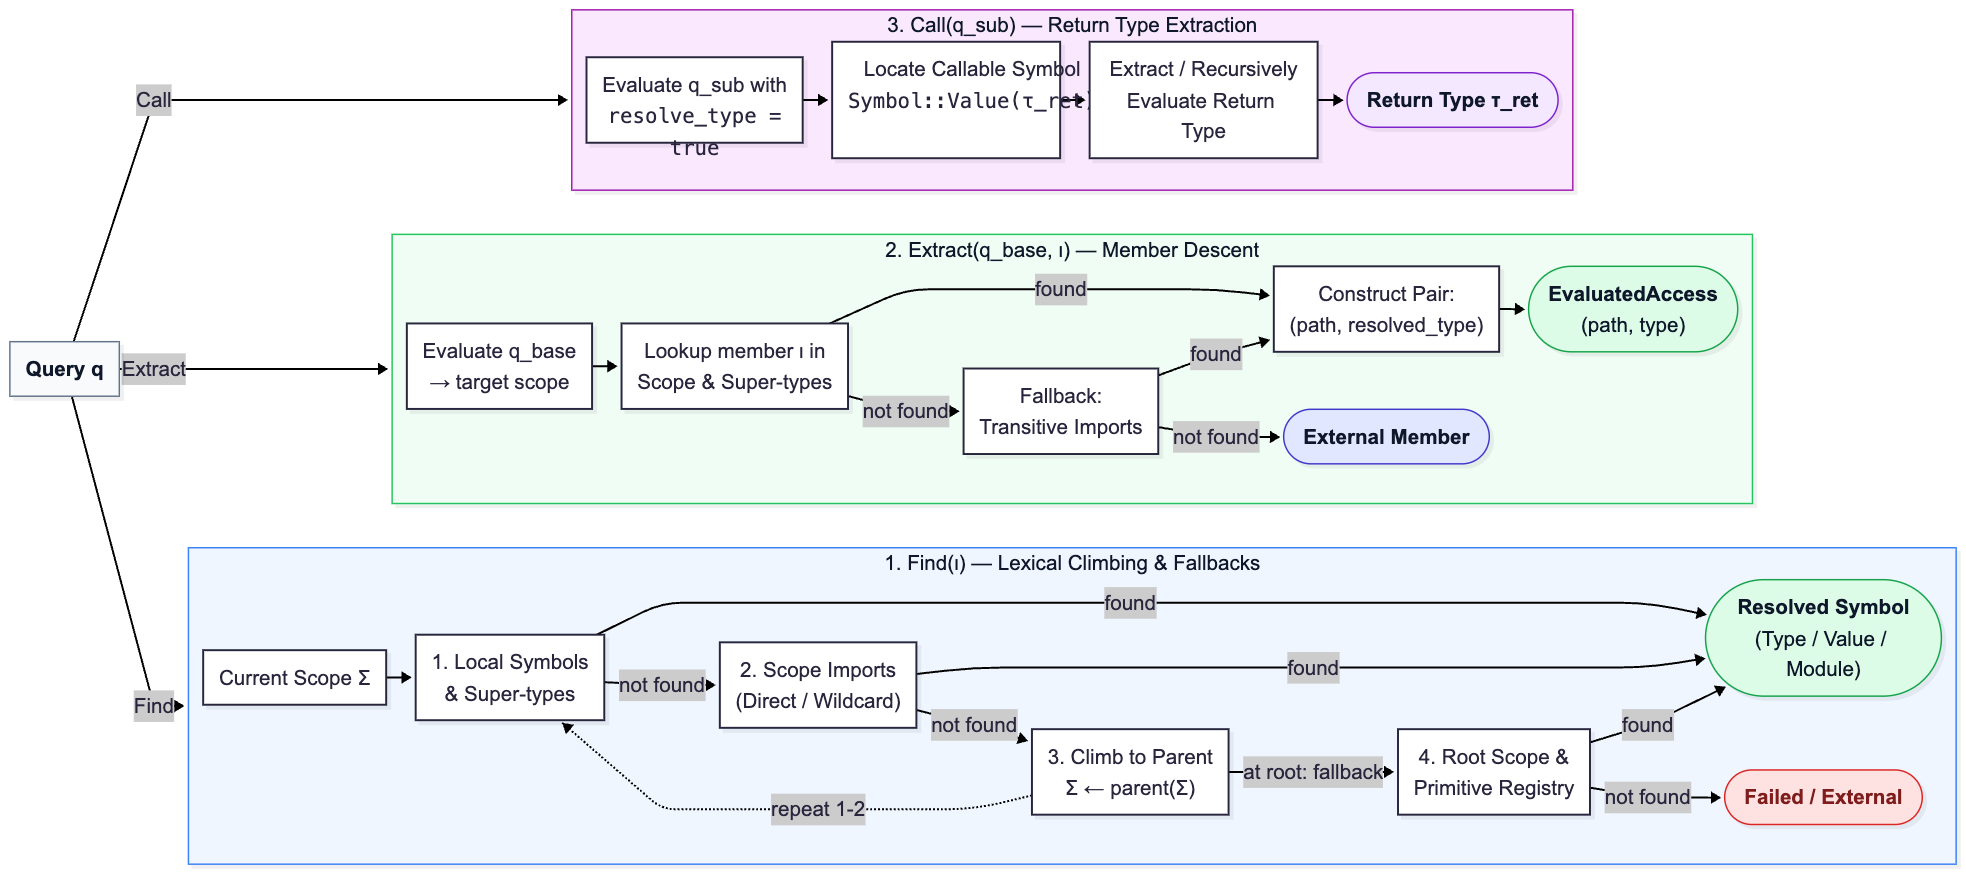
\includegraphics[width=\textwidth]{images/name_resolution/query_execution_flow.png}
  \caption{Evaluation pathways of resolution queries: parallel execution tracks for lexical climbing ($\texttt{Find}$), structural member descent ($\texttt{Extract}$), and return type extraction ($\texttt{Call}$).}
  \label{fig:query_execution_flow}
\end{figure}

Cycle detection in lexical climbing and symbol evaluation is tracked
via composite keys combining the active scope identifier and the symbol name:
$$k_{\text{query}} = \langle \Sigma, \text{base}(q) \rangle \in \Sigma \times \mathcal{I}$$
and symbol keys:
$$k_{\text{sym}} = \langle \Sigma, \iota \rangle \in \Sigma \times \mathcal{I}$$
This contextual scoping prevents false cycle alarms across homonymous
symbols in unrelated scopes, while reliably terminating self-referential
assignments (such as Python $x = x[k]$) and cyclic re-exports.

When evaluating a $\texttt{Find}(\iota)$ query starting from scope
$\Sigma_0$, the executor implements the following algorithm:

\begin{enumerate}
  \item \textbf{Special Keywords}: If $\iota$ is \texttt{super} or
    \texttt{super()}, invoke the super-type resolver. If $\iota$ is
    \texttt{Self}, resolve to the target type of the current
    \texttt{impl} block context.

  \item \textbf{Local Symbol Search}: Search $\Sigma_0$'s symbol
    table for $\iota$. If found, resolve the symbol (see below).
    Additionally, search inherited scopes via super-types (Section
    \ref{sec:inheritance_resolution}).

  \item \textbf{Import Search}: Iterate over $\Sigma_0$'s imports:
    \begin{itemize}
      \item If an import path ends with $\iota$ (direct import), attempt
        to resolve the full path globally via \texttt{find\_global}.
        If the path is not found in the workspace, classify it as
        \texttt{TypeRef::External}.
      \item If an import is a wildcard (\texttt{*}), construct a
        specific path by replacing the wildcard with $\iota$ and attempt
        global resolution.
    \end{itemize}

  \item \textbf{Climb}: Set $\Sigma_0 \leftarrow
    \text{parent}(\Sigma_0)$ and repeat from step 2.

  \item \textbf{Root Fallback}: If the root scope is reached without
    a match, attempt a global search from the root using \texttt{find\_global}.

  \item \textbf{Primitive Check}: If the global search also fails,
    consult the Primitive Registry ($\mathcal{P}$). If $\iota$ is a
    known primitive type for the current language, return
    \texttt{TypeRef::Primitive($\iota$)}.

  \item \textbf{Failure}: Return \texttt{TypeRef::Failed}.
\end{enumerate}

\subsubsection{Global Path Navigation: \texttt{find\_global}}

The function \texttt{find\_global} resolves absolute qualified paths
by navigating from the root scope downward. For a path $\pi = \langle \iota_1,
\iota_2, \ldots, \iota_k \rangle$, it looks up $\iota_1$ in the root scope,
navigates to the resulting scope, looks up $\iota_2$, and so on. If at
any point a segment is not found, the function returns \texttt{None},
and the caller may classify the reference as \texttt{External}.

A special case handles single-segment paths: if $k = 1$ and $\iota_1$ is
recognized by the Primitive Registry, the function returns
\texttt{TypeRef::Primitive} directly.

\subsection{Member Extraction and Inheritance ($\texttt{Extract}$)}
\label{sec:inheritance_resolution}

When evaluating an $\texttt{Extract}(q, \iota)$ query, the executor first
evaluates $q$ to obtain a target scope, then searches for member
$\iota \in \mathcal{I}$
within that scope. If $\iota$ is not found directly, the search proceeds
through the type's super-type hierarchy.

When evaluating super-type references of a structured type with scope
$\Sigma_C$, resolution initiates from $\Sigma_C$ itself so that formal
type parameters (e.g., $T$) declared locally are accessible.
To prevent combinatorial explosion in multiple inheritance hierarchies
(such as classes implementing dozens of interfaces, where naive recursive
exploration incurs factorial complexity $\mathcal{O}(b!)$), the resolver
employs a memoization sentinel:
$$\mathcal{M}(\Sigma_C) \leftarrow \emptyset$$
Before recursively exploring the base types of $\Sigma_C$, an empty set
is inserted as a sentinel in $\mathcal{M}(\Sigma_C)$. Any re-entrant inquiry
for $\Sigma_C$'s super-scopes during base-type evaluation immediately
terminates in $\mathcal{O}(1)$, allowing lexical climbing to ascend
directly to $\text{parent}(\Sigma_C)$ to find base types without divergence.
Once direct super-types are evaluated, $\mathcal{M}(\Sigma_C)$ is updated
with the resolved ancestor scopes. A decoupled visitation set isolates
super-scope exploration from the caller's query stack. This reduces
inheritance traversal from exponential complexity to a linear depth-first
search over ancestor scopes:
$$\mathcal{O}(|V_{\text{supers}}| + |E_{\text{supers}}|)$$
guaranteeing instant convergence even on complex multi-interface hierarchies.

The function \texttt{find\_symbol\_in\_scope\_and\_supers} implements
the following algorithm:

\begin{enumerate}
  \item Search the target scope's symbol table for $\iota$. If found,
    return the resolved symbol.
  \item Retrieve or resolve the ancestor scopes via $\mathcal{M}(\Sigma)$.
  \item For each ancestor scope in depth-first order:
    \begin{enumerate}
      \item Search the ancestor scope's symbol table for $\iota$.
      \item If found, return the resolved symbol.
    \end{enumerate}
  \item A \texttt{visited} set prevents infinite loops in the presence
    of diamond inheritance or circular trait dependencies.
\end{enumerate}

\paragraph{Nominal Projection Fallback for External and Dynamic Members}
If member $\iota$ is not found within the candidate scopes, their super-type
hierarchies, or through transitive imports, the executor avoids prematurely
discarding the reference. When the base receiver evaluates to a known path
($\text{Resolved}(\pi)$, $\text{External}(\pi)$, or $\text{Unresolved}(\pi)$),
the executor synthesizes an updated reference by appending $\iota$ to the path:
$$\pi' = \pi \cup \langle \iota \rangle$$
producing $\text{EvaluatedAccess}(\text{Base}(\pi), \text{Base}(\pi'))$.
This conservative fallback guarantees that references to external library members
(such as \texttt{requests.Session.get}) or unannotated dynamic attributes are
preserved, enabling Phase 3 to project valid architectural dependency edges toward
external endpoints.

\subsubsection{Rust Deref Coercion as Inheritance}

Rust does not have classical class inheritance, but the \texttt{Deref} trait
provides a form of implicit type coercion
\cite[Chapter~15]{klabnik_rust_2023}: if a type \texttt{T}
implements \texttt{Deref<Target = U>}, then methods and fields of \texttt{U} can
be called directly on values of type \texttt{T}. To model this within the
resolution framework, the Scope Tree construction detects
\texttt{Deref} implementations:

When registering an \texttt{ImplBlock} that implements the
\texttt{Deref} trait and contains a type alias named \texttt{Target},
the target type is added to the implementing type's
\texttt{super\_types} list. This allows the standard inheritance
resolution algorithm to search through \texttt{Deref} targets,
effectively treating \texttt{Deref} coercion as a form of structural
inheritance.

\subsubsection{Transitive Import Resolution in Modules}
\label{sec:transitive_imports}

When the \texttt{transitive\_imports} configuration flag is enabled
(e.g., for Python), the resolver can follow import chains through
intermediate modules. This models the common Python pattern of
importing and re-exporting names through \texttt{\_\_init\_\_.py} files.

The function \texttt{resolve\_via\_transitive\_imports} is invoked
when a member $\iota$ is not found directly in a module scope. It
inspects the module's imports for entries that match $\iota$ (either by
name or via a wildcard). If a matching import is found, the import
path is resolved globally. If the path points to a known workspace
entity, the resolution succeeds; otherwise, the reference is
classified as \texttt{External}.

Wildcard imports are handled by removing the terminal \texttt{*} token
before appending the queried member name $\iota$. Mutual recursion between
global path lookup and transitive import exploration is prevented by
maintaining dedicated visitation guards: a path set $V_{\text{global}} \subseteq \Pi$
for global navigation and a composite set $V_{\text{trans}} \subseteq \Sigma \times \mathcal{I}$
for module-member re-exports.

This mechanism is controlled per-language: it is enabled for Python
(where re-exports are idiomatic) and disabled for languages like Java
and Rust (where import semantics are strictly non-transitive).

\subsection{Call Query Evaluation ($\texttt{Call}$)}
\label{sec:call_query_evaluation}

The evaluation of invocation queries in Phase 2b mirrors the
operational distinction between
type-level queries and behavioral call targets:

\begin{enumerate}
  \item \textbf{Type-Level Evaluation ($\texttt{Call}(q)$)}: When
    evaluating an explicit
    $\texttt{Call}(q)$ query, the executor calls
    $\texttt{evaluate\_query}$ with the flag
    $\texttt{resolve\_type} = \text{true}$. The sub-query $q$ is
    evaluated to locate the callee's
    symbol in the Scope Tree. When a callable symbol is found
    (represented as $\texttt{Symbol::Value}(\tau_{\text{ret}})$
    carrying the declared or inferred return type), the executor
    unpacks and returns $\tau_{\text{ret}}$
    rather than the callee's own identifier path. If
    $\tau_{\text{ret}}$ is itself a deferred
    \texttt{ResolutionQuery}, it is evaluated recursively within the
    callee's scope.
    This enables seamless type propagation across method chains of
    arbitrary depth (e.g.,
    \texttt{repo.find().as\_dto()}).
  \item \textbf{Behavioral Call Target Resolution
    ($b.\text{calls}$)}: Conversely, when evaluating
    the statement-level invocation targets of an executable block ($c
    \in b.\text{calls}$),
    the executor invokes $\texttt{evaluate\_typeref}$ with
    $\texttt{resolve\_type} = \text{false}$.
    Under this setting, locating a callable symbol preserves its
    canonical symbol path
    (e.g., $\texttt{Resolved}([\text{app}, \text{OrderService},
    \text{validate}])$) instead of collapsing
    resolved target is subsequently passed through constructor
    redirection (Section \ref{sec:constructor_redirection}) and
    semantic cast disambiguation (Section
    \ref{sec:call_cast_disambiguation}) to handle class
    instantiations or type casts masquerading as calls, and finally
    emitted as an edge in the dependency graph during Phase 3.
\end{enumerate}

\subsubsection{Constructor Redirection}
\label{sec:constructor_redirection}

A subtle but vital semantic discrepancy in static analysis occurs during object
instantiation and constructor execution. In source code across major programming
languages, object creation is syntactically expressed by invoking or referencing
the structured type itself:
\begin{itemize}
  \item In Java and C++: \texttt{new Car(engine)} or direct stack initialization
    \texttt{Car car(engine)};
  \item In Python: \texttt{car = Car(engine)};
  \item In JavaScript / TypeScript: \texttt{new Car(engine)}.
\end{itemize}

During syntactic extraction (Phase 1), the expressions recorded in
\texttt{Block::instantiates}
and \texttt{Block::calls} capture the nominal identifier of the
target class (e.g.,
$\text{Unresolved}(\langle \texttt{Car} \rangle)$). When Phase 2
evaluates this query,
standard lexical lookup initially yields the structured type itself:
$\text{Resolved}(\langle \texttt{models}, \texttt{Car} \rangle)$.

However, from an architectural and behavioral standpoint, invoking an
object constructor
is fundamentally an invocation of executable behavior rather than
merely a passive
type-level reference. If the resolution engine terminated at the
class node, Phase 3
(Graph Construction) would only be able to emit a generic type
dependency, obscuring
the direct call coupling toward the constructor method.

To bridge this syntactic gap, the function
\texttt{redirect\_to\_constructor} inspects
all resolved references in \texttt{Block::calls} and
\texttt{Block::instantiates}:

\begin{enumerate}
  \item If the reference evaluates to a structured type
    ($\text{Resolved}(\pi)$), the
    executor retrieves the corresponding type scope in the Scope Tree
    $\mathcal{E}$ via
    \texttt{find\_scope\_for\_type}.
  \item It checks the scope's symbol table for known constructor
    naming conventions
    across the supported languages:
    $$\mathcal{I}_{\text{ctor}} = \{ \texttt{"\_\_init\_\_"},
    \texttt{"constructor"}, \text{last}(\pi) \}$$
    capturing Python's \texttt{\_\_init\_\_}, TypeScript's
    \texttt{constructor}, and
    Java/C++ constructors that match the class name itself.
  \item If an explicit constructor method is found, the resolved path
    is specialized
    by appending the constructor identifier:
    $$\pi_{\text{ctor}} = \pi \cup \langle \iota_{\text{ctor}} \rangle$$
    transforming $\text{Resolved}(\langle \texttt{models},
    \texttt{Car} \rangle)$ into
    $\text{Resolved}(\langle \texttt{models}, \texttt{Car},
    \texttt{\_\_init\_\_} \rangle)$.
  \item If the reference is a compound
    $\text{EvaluatedAccess}(\tau_{\text{base}}, \tau_{\text{inner}})$,
    the redirection recursively applies to $\tau_{\text{inner}}$,
    preserving the base
    access while updating the resolved method target.
  \item If the class defines no explicit constructor (relying on
      synthesized or default
    language semantics), the reference remains unaltered, pointing
    directly to the
    structured type.
\end{enumerate}

This mechanism allows Phase 3 to cleanly differentiate between pure type-level
instantiations and explicit behavioral constructor calls, emitting
\texttt{DependencyKind::ConstructorCall} whenever a dedicated
constructor method is
invoked.

\subsubsection{Disambiguating Function Invocations and Type Coercions}
\label{sec:call_cast_disambiguation}

A notorious grammatical challenge in parsing languages like C is the
syntactic ambiguity between function calls and type casts \cite{aho_compilers_2007}.
Consider a parenthesized expression of the form:
\begin{equation}
  (T)(e)
\end{equation}
In traditional C compiler frontends (such as GCC or Clang), this ambiguity is
resolved during lexical analysis via the classic ``lexer hack'': the scanner
queries the symbol table and yields distinct token types (\texttt{TYPE\_NAME}
versus \texttt{IDENTIFIER}) depending on whether $T$ has been registered as a
\texttt{typedef}.

In contrast, Tree-sitter parses source files in isolation without lexical
feedback from an active symbol table. Consequently, Tree-sitter's context-free
parsing tables interpret $(T)(e)$ as a \texttt{call\_expression} whenever $T$ is
an arbitrary typedef identifier or when the operand $e$ is itself parenthesized,
classifying $(T)$ as a parenthesized callable function and $(e)$ as its argument list.

Because OmniDeps strictly separates local syntactic extraction (Phase 1) from
global semantic resolution (Phase 2), the framework does not attempt to resolve
this ambiguity through ad-hoc syntactic heuristics during CST traversal. Instead,
Phase 1 faithfully unrolls the parenthesized callee (recording $T$ in
$\mathcal{B}.\text{calls}$), deferring disambiguation to the query execution
phase ($\rho_{\text{exec}}$) where the global Scope Tree $\mathcal{E}$ is fully
materialized.

During Phase 2b, the resolution engine inspects every call target $c \in \mathcal{B}.\text{calls}$.
Crucially, rather than embedding hardcoded language switches (e.g., \texttt{if is\_c}),
OmniDeps addresses this variance through its declarative resolution configuration
$\mathcal{K}$ (Section \ref{sec:resolution_config}):
\begin{itemize}
  \item In object-oriented languages like Python and C++, types are first-class
    callable entities (\texttt{callable\_types = true}), where invoking a class
    syntactically executes an instance constructor.
  \item In procedural languages like C, types are fundamentally non-callable
    entities (\texttt{callable\_types = false}): C possesses neither user-defined
    constructors nor callable operator overloading (\texttt{operator()}).
\end{itemize}

Formally, let $\tau = \rho_{\text{exec}}(c, s)$ be the evaluated call target within
lexical scope $s$, and let $\mathcal{K}_s = \mathcal{K}(\text{language}(\mathcal{E}, s))$
be the active resolution configuration. The engine evaluates:
\begin{equation}
  \text{is\_type\_or\_alias}(\tau) = 
  \begin{cases}
    \text{true} & \text{if } \tau \in \mathcal{P} \\
                & \quad \lor \ \text{lookup}(\mathcal{E}, \tau) \in \{ \text{Symbol::Type}, \text{Symbol::TypeAlias} \} \\
    \text{false} & \text{otherwise}
  \end{cases}
\end{equation}
where $\mathcal{P}$ is the Primitive Registry and $\text{lookup}(\mathcal{E}, \tau)$
retrieves the symbol declaration from the Scope Tree. If $\neg \mathcal{K}_s.\texttt{callable\_types}$
and $\text{is\_type\_or\_alias}(\tau)$ holds true, the reference cannot semantically
represent an executable function call. The executor reclassifies the reference as a
type cast:
\begin{equation}
  \mathcal{B}.\text{type\_casts} \gets \mathcal{B}.\text{type\_casts} \cup \{ \tau \}, \quad \mathcal{B}.\text{calls} \gets \mathcal{B}.\text{calls} \setminus \{ \tau \}
\end{equation}

This parameter-driven disambiguation guarantees that Phase 3 emits a precise
\texttt{DependencyKind::CastsTo} edge for expressions such as \texttt{(MyInt)(val)} or
\texttt{(int)(5.0)}, while genuine function calls enclosed in protective parentheses
(such as \texttt{(add)(a, b)} or \texttt{(square\_func)(a)}) resolve to $\text{Symbol::Value}$
and correctly remain in $\mathcal{B}.\text{calls}$. Furthermore, because this
behavior is governed declaratively by $\mathcal{K}$, the core resolution engine remains
strictly language-agnostic.

\subsection{Dual-Tracking of Access Chains: \texttt{EvaluatedAccess}}
\label{sec:evaluated_access}

A fundamental architectural challenge in static dependency extraction
arises when
resolving chained member expressions (such as field dereferences
  \texttt{order.customer.address}
or method invocations \texttt{conn.getMetaData().getTables()}). Such
expressions impose
a dual semantic requirement:

\begin{enumerate}
  \item \textbf{Navigational / Typing Requirement}: To iteratively
    resolve subsequent
    segments in an access chain (e.g., finding the member
      \texttt{address} within
    \texttt{customer}), the static engine requires the
    \textit{structural type} of
    the receiver (i.e., the class \texttt{Customer}, its Scope Tree
      node, and its
    declared fields and methods).
  \item \textbf{Architectural Dependency Requirement}: When
    projecting the resolved
    IR into the architectural dependency graph $\mathcal{G} = (V, E)$ in Phase 3
    (Chapter \ref{ch:graph_construction}), the analyzer requires the
    identity of the
    \textit{concrete physical component accessed} (e.g., the field
    \texttt{Order::customer}),
    so as to emit fine-grained behavioral dependencies
    (\texttt{Accesses}, \texttt{Calls})
    rather than coarse, uninformative type-level links.
\end{enumerate}

If the resolution engine resolved an access expression solely to its
underlying type
(discarding the accessed field and yielding only \texttt{Customer}),
the graph generator
would lose the identity of the member being accessed. Conversely, if
the engine returned
only the accessed member symbol without its resolved type, it would
lack the type context
necessary to locate subsequent members in the chain.

To eliminate this trade-off, OmniDeps introduces the compound resolution state:
$$\text{EvaluatedAccess}(\tau_{\text{path}}, \tau_{\text{type}})$$
where:
\begin{itemize}
  \item $\tau_{\text{path}}$ captures the accumulated qualified path
    of the concrete
    syntactic component accessed in the source code (e.g.,
    $\text{Resolved}(\langle \texttt{Order}, \texttt{customer} \rangle)$);
  \item $\tau_{\text{type}}$ captures the evaluated structural type
    of that component
    (e.g., $\text{Resolved}(\langle \texttt{Customer} \rangle)$), supplying the
    target scope for subsequent member resolution.
\end{itemize}

During query execution in \texttt{executor.rs},
\texttt{EvaluatedAccess} operates
through an unwrapping and re-wrapping protocol:
\begin{itemize}
  \item When evaluating an $\texttt{Extract}(q, m)$ query, the
    executor evaluates the
    base sub-query $q$. If $q$ yields an
    $\text{EvaluatedAccess}(\tau_{\text{base}},
    \tau_{\text{inner}})$, the executor unwraps $\tau_{\text{inner}}$
    to locate the
    target \texttt{ScopeId} via \texttt{find\_scope\_for\_type},
    while preserving
    $\tau_{\text{base}}$ as the active access prefix.
  \item Once member $m$ is located within the target scope or its
    super-type hierarchy
    (producing resolved symbol $\tau_{\text{res}}$), the executor
    updates the access chain:
    $$\text{EvaluatedAccess}(\tau_{\text{base}}, \tau_{\text{res}})$$
    If the base was a simple type reference rather than an existing
    chain, the parent
    itself is encapsulated as the base access.
  \item When resolving symbols in \texttt{symbol\_to\_typeref}, looking up a
    \texttt{Symbol::Value} or \texttt{Symbol::TypeAlias} with
    $\text{resolve\_type} =
    \text{true}$ automatically packages the symbol's declared path
    and its resolved
    type into an \texttt{EvaluatedAccess} pair.
  \item Global path resolution (\texttt{find\_global}) similarly
    encapsulates the
    final scope into $\text{EvaluatedAccess}(\text{Resolved}(\pi),
    \text{Resolved}(\pi))$.
\end{itemize}

This mechanism bridges the semantic gap between Phase 2 and Phase 3: the graph
construction engine can simultaneously project an \texttt{Accesses}
or \texttt{Calls}
edge to $\tau_{\text{path}}$ and a \texttt{TypedAs} dependency to
$\tau_{\text{type}}$,
guaranteeing complete architectural fidelity without loss of
behavioral information. Figure \ref{fig:evaluated_access_tracking} traces the progressive accumulation of paths and types across a member access chain.

\begin{figure}[htpb]
  \centering
  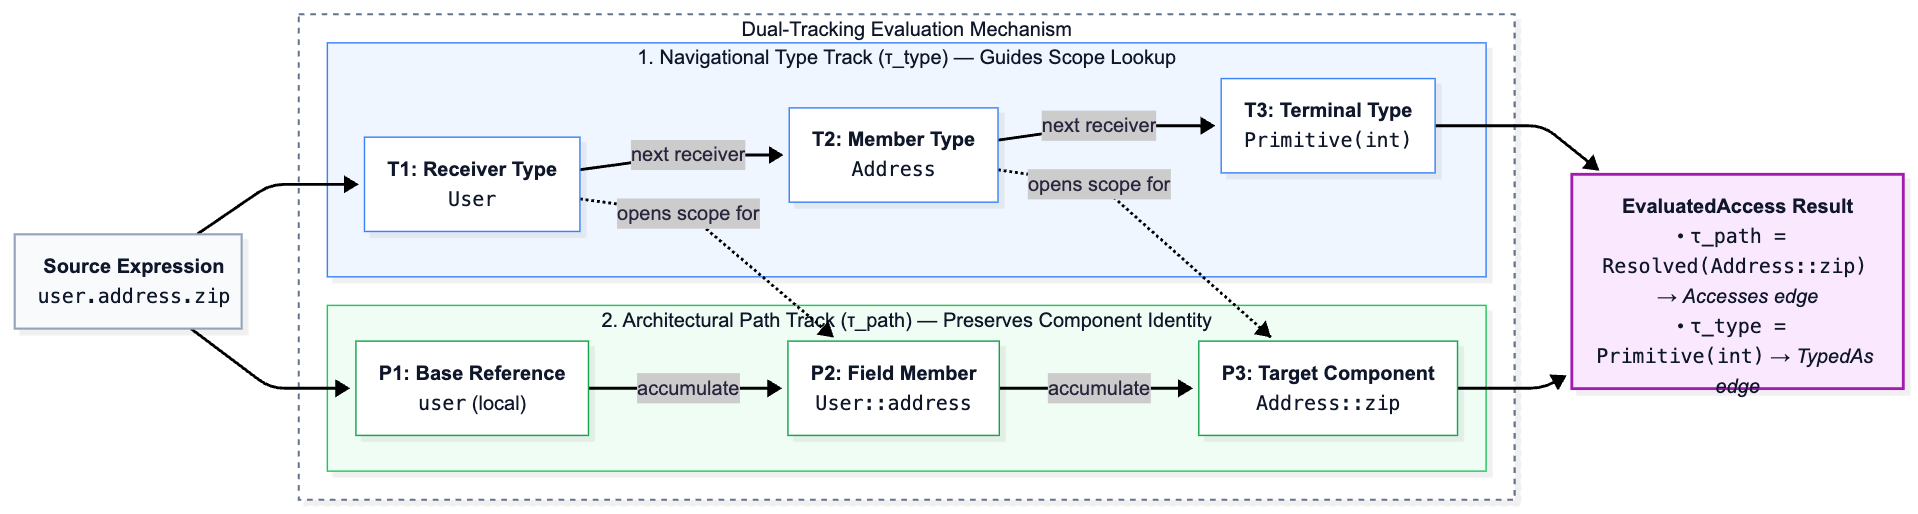
\includegraphics[width=\textwidth]{images/name_resolution/evaluated_access_tracking.png}
  \caption{Dual-tracking evaluation of chained member access \texttt{user.address.zip}: maintaining the concrete syntactic access path alongside the resolved structural type for architectural dependency projection.}
  \label{fig:evaluated_access_tracking}
\end{figure}

\subsection{Parametric Polymorphism and Generic Resolution}
\label{sec:generics_resolution}

Parametric polymorphism (generics in Java, Rust, and Python, or templates
in C++) introduces an orthogonal dimension to static symbol resolution:
it decouples the structural definition of an algorithmic abstraction from
the concrete type arguments supplied at instantiation sites.

To formalize parametric polymorphism without sacrificing language agnosticism,
the Intermediate Representation distinguishes between generic application and
type parameter declarations:
\begin{align*}
  \tau_{\text{app}} &= \text{Generic}(\tau_{\text{base}}, \vec{\tau}_{\text{args}}) \\
  \tau_{\text{var}} &= \text{TypeVar}(\iota, \vec{\tau}_{\text{bounds}})
\end{align*}

\subsubsection{Resolution of Disjunctive Types: \texttt{Union}}
\label{sec:union_resolution}

In heterogeneous, multi-language codebases, type references frequently
exhibit disjunctive characteristics. To faithfully capture
these constructs without premature approximation, the intermediate
representation introduces the compound type reference:
$$\text{Union}(\vec{\tau}) = \text{Union}(\langle \tau_1, \tau_2, \ldots, \tau_k \rangle)$$
Such variants originate during syntactic extraction (Phase 1) in two
primary scenarios:
\begin{enumerate}
  \item \textbf{Explicit Union Annotations}: In dynamically typed languages
    with gradual typing features (such as Python's \texttt{int | str} or
    \texttt{Union[User, Guest]}), an identifier can evaluate to
    multiple distinct types at runtime.
  \item \textbf{Multi-Branch Return Type Inference}: When inferring the return
    type of unannotated functions exhibiting multiple return statements with
    differing types.
\end{enumerate}

During Phase 2a (Query Building), the substitution function
\texttt{substitute\_type} applies intra-procedural lexical substitutions
recursively across each constituent member of the union.

During Phase 2b (Query Execution), query evaluation distributes homomorphically
over the union variants in \texttt{evaluate\_typeref}:
$$\rho_{\text{exec}}(\text{Union}(\{ \tau_1, \tau_2, \ldots, \tau_k \})) =
\text{Union}(\{ \rho_{\text{exec}}(\tau_1), \rho_{\text{exec}}(\tau_2), \ldots, \rho_{\text{exec}}(\tau_k) \})$$
Each inner reference $\tau_i$ is evaluated independently against the Scope Tree
$\mathcal{E}$ and may resolve to any valid post-resolution state (such as
$\texttt{Resolved}$, $\texttt{Primitive}$, or $\texttt{External}$).

Finally, during Phase 3 (Graph Construction, Chapter \ref{ch:graph_construction}),
the dependency projector processes \texttt{TypeRef::Union} by flattening its
underlying targets (\texttt{flat\_map}). Rather than heuristically selecting a
single candidate or dropping ambiguous alternatives, OmniDeps emits dependency
edges toward all resolved targets present within the union. This conservative
strategy ensures that all potential behavioral and structural couplings induced
by polymorphic type choices are faithfully represented in the architectural
dependency graph.

\subsubsection{Phantom Scopes in the Scope Tree}

When building the Scope Tree during Phase 2a, registering a generic structured
type or function allocates synthetic scopes termed \textit{Phantom Scopes}
($\Sigma_{\text{phantom}}$) within the arena for each declared type parameter
$\theta = \langle \iota, \vec{\tau}_{\text{bounds}} \rangle$. A phantom scope
is characterized by:
\begin{enumerate}
  \item $\text{is\_phantom} = \text{true}$, marking it as an ephemeral lexical
    placeholder that does not generate independent vertices during graph construction;
  \item $\text{name} = \langle \iota \rangle$, binding the parameter identifier;
  \item $\text{super\_types} = \vec{\tau}_{\text{bounds}}$, recording the upper
    bound constraints (e.g., interface implementations or trait bounds).
\end{enumerate}

Within the enclosing lexical scope of the generic declaration, $\iota$ is
defined as $\texttt{Symbol::Type}(\text{TypeRef::TypeVar}(\iota, \vec{\tau}_{\text{bounds}}))$.
Consequently, method signatures and local variable declarations inside the
generic entity can refer to $\iota$ as a valid type.

\subsubsection{Two-Phase Bound Lifecycle}

Constraint bounds undergo a two-phase evaluation lifecycle:
\begin{enumerate}
  \item \textbf{Lexical Binding (Phase 2a)}: The bounds $\vec{\tau}_{\text{bounds}}$
    are recorded as raw or locally substituted type references.
  \item \textbf{Bound Evaluation (Phase 2b)}: During query execution,
    $\texttt{evaluate\_typeref\_inner}$ evaluates each bound $\tau \in \vec{\tau}_{\text{bounds}}$
    against the Scope Tree. If a bound resolves to a known structured type
    ($\text{Resolved}(\pi)$ or $\text{External}(\pi)$), the phantom scope
    inherits the member suite of that bound.
\end{enumerate}

\subsubsection{Candidate Scopes and Multi-Bound Dispatch}

When an expression accesses a member on a target whose evaluated type is
$\text{TypeRef::TypeVar}(\iota, \vec{\tau}_{\text{bounds}})$, member lookup
cannot be restricted to a single nominal scope. Instead, the function
\texttt{find\_candidate\_scopes\_for\_type} computes a set of candidate scopes:
$$\text{scopes}(\text{TypeVar}(\iota, \vec{\tau}_{\text{bounds}})) =
\bigcup_{\tau_b \in \vec{\tau}_{\text{bounds}}} \text{scopes}(\tau_b)$$
This multi-scope dispatch allows variables constrained by compound bounds
(for instance, $T: \text{Display} + \text{Clone}$ in Rust) to resolve members
originating from any of the specified traits. If any candidate scope provides
the queried member, resolution succeeds.

\subsubsection{Type Parameter Substitution ($\sigma$)}

When a generic type application $\text{Generic}(\tau_{\text{base}}, \vec{\tau}_{\text{args}})$
is accessed (e.g., calling a method on an instance of \texttt{Repository<User>}),
the receiver scope is determined by evaluating $\tau_{\text{base}}$ to locate
the underlying generic definition $\mathcal{S}$ with formal parameters
$\vec{\theta} = \langle \theta_1, \ldots, \theta_k \rangle$.

Upon retrieving a member whose signature involves formal type parameters,
the engine constructs a substitution mapping:
$$\sigma = [ \theta_1.\iota \mapsto \tau_{\text{args}}[1], \ldots, \theta_k.\iota \mapsto \tau_{\text{args}}[k] ]$$
The helper function \texttt{instantiate\_generic\_member\_type} applies $\sigma$
recursively across the member's return type or field type:
\begin{align*}
  \sigma(\text{TypeVar}(\iota, \_)) &=
  \begin{cases}
    \tau_{\text{arg}} & \text{if } (\iota \mapsto \tau_{\text{arg}}) \in \sigma \\
    \text{TypeVar}(\iota, \_) & \text{otherwise}
  \end{cases} \\
  \sigma(\text{Generic}(\tau_b, \vec{\tau}_a)) &= \text{Generic}(\sigma(\tau_b), \vec{\sigma}(\vec{\tau}_a)) \\
  \sigma(\text{Union}(\vec{\tau})) &= \text{Union}(\vec{\sigma}(\vec{\tau}))
\end{align*}
Thus, if \texttt{Repository<T>} defines \texttt{find(id: ID) -> T}, evaluating
\texttt{repo.find(1)} on a \texttt{Repository<User>} substitutes $T \mapsto \text{User}$,
resolving the invocation's return type directly to \texttt{User}.

\subsubsection{Chained Access Propagation}

When evaluating multi-segment dot-accesses (e.g., \texttt{user.profile.settings}),
the intermediate structural transitions are preserved using
$\text{TypeRef::EvaluatedAccess}(\tau_{\text{path}}, \tau_{\text{type}})$.
This composite reference retains both the evaluated path and the resolved
structural type, enabling Phase 3 to emit dependency edges for every
intermediate component participating in the access chain.

\section{Implementation Block Flattening}
\label{sec:impl_flattening}

During Scope Tree construction, implementation blocks
(\texttt{ImplBlock}) are flattened into the scope of their target
type. This process unifies the syntactic separation of declaration
and definition (common in languages like Rust with \texttt{impl} blocks,
and C++ with out-of-line method definitions) with the conceptual unity
of a structured type and its member suite.

The flattening algorithm operates as follows:
\begin{enumerate}
  \item \textbf{Target Type Identification}: Extracts the canonical target name
    from \texttt{ib.impl\_for}.
  \item \textbf{Scope Association}: Searches for the target
    structured type's scope
    within the parent module scope. If not found locally, a
    \textbf{global fallback search}
    scans all arena scopes for a matching name (e.g., handling
      cross-unit C++ \texttt{.h}/\texttt{.cpp}
    separations or multi-file Rust modules).
  \item \textbf{Self-Type Alias Injection}: If a
    \texttt{self\_type\_keyword} is configured
    for the language (e.g., \texttt{"Self"} for Rust), a
    \texttt{Symbol::TypeAlias} pointing
    to \texttt{ib.impl\_for} is defined in the target type's scope.
  \item \textbf{Member Transfer}: All methods declared inside the
    \texttt{ImplBlock}
    are registered as callable symbols within the target type's
    scope, enabling subsequent
    lexical and member searches to discover them directly.
  \item \textbf{Associated Types and Nested Definitions}: All nested
    types and type aliases
    declared in the block are similarly absorbed into the target type scope.
  \item \textbf{Trait Handling vs.\ Deref Coercion}:
    \begin{itemize}
      \item Standard trait implementations
        (\texttt{ib.implements\_trait}) are \textit{not}
        treated as structural inheritance in the Scope Tree; instead,
        the trait reference is
        preserved directly on the IR \texttt{ImplBlock} node,
        resolved to its canonical symbol
        during Phase 2b (\texttt{execute\_impl\_block}), and used in
        Phase 3 (Chapter \ref{ch:graph_construction})
        to emit an explicit $\text{TargetType}
        \xrightarrow{\text{Implements}} \text{Trait}$
        architectural dependency.
      \item The sole exception is Rust's \texttt{Deref} trait: when
        an \texttt{ImplBlock}
        implements \texttt{Deref} and defines an associated type
        alias \texttt{type Target = U},
        the target type $U$ is appended to the implementing type's
        \texttt{super\_types} list
        (Section \ref{sec:inheritance_resolution}). This allows the
        inheritance search algorithm
        to naturally traverse method dereferencing chains without
        altering general trait semantics.
    \end{itemize}
\end{enumerate}

Within the Scope Tree $\mathcal{E}$, implementation blocks do not
maintain separate scope nodes;
their member definitions are directly amalgamated into the target
type's lexical scope. However,
within the intermediate representation ($\vec{\mathcal{M}} \in
\mathcal{D}$), the \texttt{ImplBlock}
structures remain preserved as first-class architectural containers,
ensuring that Phase 3 can
reliably extract trait realization dependencies and method nesting relations.

\section{The Primitive Registry ($\mathcal{P}$)}
\label{sec:primitive_registry}

To prevent built-in types (e.g., \texttt{int}, \texttt{bool},
\texttt{String}, \texttt{void}, \texttt{usize}) from being classified
as \texttt{Failed} or \texttt{External}, the analyzer maintains a
data-driven Primitive Registry. The registry is loaded from a JSON
file (\texttt{primitives.json}) that maps language names to lists of
primitive type identifiers:

\begin{verbatim}
{
  "rust": ["i8", "i16", "i32", "i64", "u8", ..., "bool", "str", "String", ...],
  "java": ["int", "long", "float", "double", "boolean", "char", "void", ...],
  "python": ["int", "float", "str", "bool", "None", "bytes", ...],
  ...
}
\end{verbatim}

When analyzing a multi-language workspace, the registries for all
encountered languages are merged into a single combined registry.
During query execution, the executor consults the registry as a last
resort before marking a reference as \texttt{Failed}: if the
single-segment name matches a known primitive, the reference is
resolved as \texttt{TypeRef::Primitive}.

This data-driven approach allows adding primitives without modifying
the resolver's code, and ensures that common types like \texttt{int}
or \texttt{bool} are correctly classified regardless of the language context.

\section{Resolution Configuration ($\mathcal{K}$)}
\label{sec:resolution_config}

Due to the semantic differences between supported languages, the
resolution phase is parameterized by a per-language configuration.
Table \ref{tab:resolution_config} summarizes the key parameters and
their effects.

\begin{table}[htpb]
  \centering
  \small
  \begin{tabularx}{\textwidth}{|l|l|X|}
    \hline
    \textbf{Parameter} & \textbf{Type} & \textbf{Effect on Resolution} \\ \hline
    \texttt{transitive\_imports} & \texttt{bool} & Enables following
    import chains through intermediate modules (Python). \\ \hline
    \texttt{self\_keyword} & \texttt{Option<String>} & Injects a
    self/this binding pointing to the enclosing type in method scopes. \\ \hline
    \texttt{self\_type\_keyword} & \texttt{Option<String>} & Injects
    a \texttt{Self} type alias in \texttt{impl} block scopes (Rust). \\ \hline
    \texttt{implicit\_first\_param\_as\_self} & \texttt{bool} &
    Treats the first method parameter as an implicit self reference
    (Python). \\ \hline
    \texttt{extract\_dynamic\_fields} & \texttt{bool} & Enables
    extraction of dynamically assigned instance fields (Python). \\ \hline
    \texttt{assignment\_type\_aliases} & \texttt{bool} & Enables
    extraction of assignment-based type definitions and TypeVar declarations (Python). \\ \hline
    \texttt{callable\_types} & \texttt{bool} & Controls whether types
    can be invoked directly as call expressions (Python, C++), as opposed to type casts (C). \\ \hline
  \end{tabularx}
  \caption{Key resolution configuration parameters and their semantic effects.}
  \label{tab:resolution_config}
\end{table}

Table \ref{tab:lang_config_matrix} shows the concrete configuration
values for each supported language.

\begin{table}[htpb]
  \centering
  \small
  \begin{tabular}{|l|c|c|c|c|c|}
    \hline
    \textbf{Parameter} & \textbf{Python} & \textbf{Rust} &
    \textbf{Java} & \textbf{C++} & \textbf{C} \\ \hline
    \texttt{transitive\_imports} & \checkmark & & & & \\ \hline
    \texttt{self\_keyword} & - & \texttt{self} & \texttt{this} &
    \texttt{this} & - \\ \hline
    \texttt{self\_type\_keyword} & - & \texttt{Self} & - & - &
    - \\ \hline
    \texttt{implicit\_first\_param\_as\_self} & \checkmark & & & & \\ \hline
    \texttt{extract\_dynamic\_fields} & \checkmark & & & & \\ \hline
    \texttt{assignment\_type\_aliases} & \checkmark & & & & \\ \hline
    \texttt{callable\_types} & \checkmark & & & \checkmark & \\ \hline
  \end{tabular}
  \caption{Concrete resolution configuration values for each
  supported language.}
  \label{tab:lang_config_matrix}
\end{table}

Through this configuration map $\mathcal{K}: \mathcal{L} \to
\mathcal{C}_{params}$, the resolution engine specializes its behavior
for each language while maintaining a strictly language-agnostic core algorithm.

\section{Termination and Convergence Guarantees}
\label{sec:resolution_termination}

A critical requirement for static architectural analysis on uncurated,
large-scale codebases is guaranteed termination and convergence. Real-world
software projects frequently exhibit cyclic patterns that risk causing infinite
recursion or combinatorial explosion during name resolution. These patterns
include circular or diamond inheritance hierarchies, mutual module re-exports,
self-referential type assignments, and wildcard package imports.

Because any target workspace produces a finite set of extracted modules
$\vec{\mathcal{M}}$, the resulting Scope Tree $\mathcal{E}$ comprises a finite
number of scopes ($|\mathcal{E}| = N < \infty$) and a finite collection of
declared symbols ($|\text{Sym}| = S < \infty$). Under the execution operator
$\rho_{\text{exec}}$, query evaluation $\texttt{evaluate\_query}(q, \Sigma)$
traverses this discrete structure. To ensure that every resolution path
terminates deterministically in a finite number of steps, the resolution engine
enforces convergence through four structural mechanisms:

\begin{enumerate}
  \item \textbf{Monotonic Lexical Climbing}: When resolving an unqualified
    identifier query $q = \text{Id}(\iota)$, the engine searches the current
    lexical scope $\Sigma$. If the identifier is not found locally, resolution
    delegates recursively to $\text{parent}(\Sigma)$. This climbing traversal
    is strictly monotonic with respect to scope depth: each ascending step
    decreases depth by one ($\text{depth}(\text{parent}(\Sigma)) = \text{depth}(\Sigma) - 1$).
    Because the Scope Tree has finite depth and terminates at the unique root
    scope $\Sigma_{\text{root}}$ (where $\text{parent}(\Sigma_{\text{root}}) = \texttt{None}$),
    lexical climbing is bounded by at most $\text{depth}(\Sigma)$ steps, either
    locating the target symbol or safely exhausting the ancestor chain.

  \item \textbf{Inheritance Traversal and Sentinel Memoization}: Querying
    members of structured types requires searching ancestor scopes along the
    class inheritance graph. This traversal introduces two distinct hazards:
    circular inheritance (such as class $A$ extending $B$ while $B$ extends $A$)
    and exponential path re-evaluation in diamond or multiple-inheritance
    hierarchies. OmniDeps addresses both hazards through the super-scope
    memoization table $\mathcal{M}$ in the execution context $\Gamma$. When
    $\texttt{resolve\_super\_scopes}$ begins inspecting a class scope $\Sigma_C$,
    it immediately records an empty sentinel entry $\mathcal{M}(\Sigma_C) \leftarrow \emptyset$
    prior to recursively evaluating any base types. If a recursive descent
    re-enters $\Sigma_C$, the sentinel is encountered immediately, yielding an
    empty set and breaking the cycle. Once all direct and transitive ancestors
    are resolved, the complete set of scopes is committed to $\mathcal{M}(\Sigma_C)$.
    Subsequent member queries for $\Sigma_C$ retrieve the cached set in $\mathcal{O}(1)$
    time. Furthermore, the active traversal maintains a visited set
    $V_{\text{scopes}} \subseteq \Sigma$, ensuring that each ancestor scope in
    the directed acyclic graph is visited at most once.

  \item \textbf{Scope-Aware Cycle Guards for Aliases and Queries}: When resolving
    type alias chains, dynamic field assignments, or re-exports, the engine
    follows references across intermediate definitions. To prevent infinite loops
    caused by self-referential assignments (such as $x = x[0]$ in dynamic scripts)
    or mutually recursive aliases, the engine maintains visited tracking sets.
    These cycle guards are indexed by composite, scope-aware keys: $k_{\text{sym}} =
    \langle \Sigma, \iota \rangle$ for symbol alias resolution and $k_{\text{query}} =
    \langle \Sigma, \text{base}(q) \rangle$ for query evaluation. Because the
    universe of valid scopes and symbol identifiers across the workspace is finite,
    the visited set monotonically expands with each dereference step. If a key is
    encountered that already exists in the set, the engine halts that branch
    immediately and yields a failed resolution ($\texttt{None}$ or $\texttt{TypeRef::Failed}$).

  \item \textbf{Transitive and Wildcard Import Decoupling}: In languages supporting
    transitive imports or wildcard package re-exports, resolving a symbol across
    modules risks oscillating indefinitely between global namespace lookups and
    transitive module traversals. To prevent mutual recursion, the engine strips
    terminal wildcard tokens before recursive lookup and partitions visitation
    tracking into separate sets: $V_{\text{global}}$ for workspace-level module
    resolution and $V_{\text{trans}}$ for transitive import chains. This separation
    ensures that each module boundary is crossed at most once per import branch.
\end{enumerate}

Through these monotonic reductions and finite-state tracking mechanisms, every
execution branch in $\texttt{evaluate\_query}$ either converges to a resolved
terminal reference or terminates upon cycle detection within finite steps.
This design guarantees both algorithmic stability and predictable execution
times across heterogeneous codebases.
